
\documentclass[11pt,letterpaper]{article}
\usepackage{amssymb,amsmath}
\usepackage{mathrsfs}
\usepackage{epsfig}
\usepackage{anysize}
\usepackage{verbatim}
\usepackage[latin1]{inputenc}
\usepackage[spanish]{babel}
%\input{macrosal}
\title{Resolviendo el problema del TSP con Recocido Simulado}
\author{V�ctor Zamora Guti�rrez}
\date{}
\begin{document}
\maketitle
\thispagestyle{empty}
El recocido simulado es una heur�stica de optimizaci�n combinatoria que sirve para resolver problemas NP duros. En esta ocasi�n, utilizamos dicha heur�stica para resolver un caso modificado del Traveling Salesman Problem (TSP): dado un conjunto de ciudades, encontrar el camino de menor peso que pase por todas las ciudades exactamente una vez.
\section{Para correr el programa}
Para correr el programa, se necesita una distribuci�n de Linux con java 8, ant y sqlite3.
Para instalar dichos programas desde ArchLinux, ejecutar:
\begin{verbatim}
$sudo pacman -S jre8-openjdk
$sudo pacman -S jdk8-openjdk
$sudo pacman -S apache-ant
$sudo pacman -S sqlite
\end{verbatim}
Teniendo esto, desde la carpeta ra�z del proyecto (la que tiene el build.xml) ejecutar:
\begin{verbatim}
$ant tsp.jar
$java -jar tsp.jar <semilla> <ciudades>
\end{verbatim}
Donde semilla es la semilla con la que se quiere correr el recocido y ciudades es un archivo que contiene una lista de ids de ciudades, separadas por una coma y un espacio.
Por ejemplo, \textit{ciudades} puede tener la siguiente l�nea:
\begin{center}
1, 5, 9, 12, 16, 22, 23, 29, 30, 31, 39, 48, 52, 56, 58, 62, 65, 66, 70, 75, 80, 84, 86, 90, 92, 94, 95, 101, 107, 117, 119, 122, 133, 135, 143, 144, 146, 147, 150, 158, 159, 160, 166, 167, 176, 178, 179, 185, 186, 188, 190, 191, 194, 198, 200, 203, 207, 209, 213, 215, 216, 220, 221, 224, 227, 232, 233, 235, 238, 241, 244, 248, 250, 254, 264, 266, 274, 276
\end{center}

Alternativamente, en la carpeta ra�z se encuentra el jar, por lo que teniendo java puede correrse el programa sin pasar por la compilaci�n.
\bigskip

Para correr las pruebas unitarias, utilizar:
\begin{verbatim}
$ant test
\end{verbatim}
Tambi�n desde la carpeta ra�z.
\bigskip

Y para generar la documentaci�n de \textit{javadoc}:
\begin{verbatim}
$ant doc
\end{verbatim}
�sta se generar� en la carpeta \textit{doc} del directorio ra�z.
\bigskip

Por �ltimo, para borrar el .jar, la documentaci�n y los archivos compilados:
\begin{verbatim}
$ant clean
\end{verbatim}
\section{Par�metros utilizados}
Para el programa, utilic� los siguientes par�metros:
\smallskip

$\epsilon = 0.0001$
\smallskip

$\epsilon_{p} = 0.0001$
\smallskip

$\varphi = 0.9 $
\smallskip

$C = 2 $

Para m�s informaci�n sobre los par�metros, leer sobre la heur�stica en los documentos de Canek Pelaez Vald�s.
\section{Gr�fica de soluciones}
La siguiente gr�fica muestra los costos de las soluciones aceptadas respecto al tiempo con el conjunto de entrada
\begin{center}
1, 5, 9, 12, 16, 22, 23, 29, 30, 31, 39, 48, 52, 56, 58, 62, 65, 66, 70, 75, 80, 84, 86, 90, 92, 94, 95, 101, 107, 117, 119, 122, 133, 135, 143, 144, 146, 147, 150, 158, 159, 160, 166, 167, 176, 178, 179, 185, 186, 188, 190, 191, 194, 198, 200, 203, 207, 209, 213, 215, 216, 220, 221, 224, 227, 232, 233, 235, 238, 241, 244, 248, 250, 254, 264, 266, 274, 276
\end{center}
\begin{center}
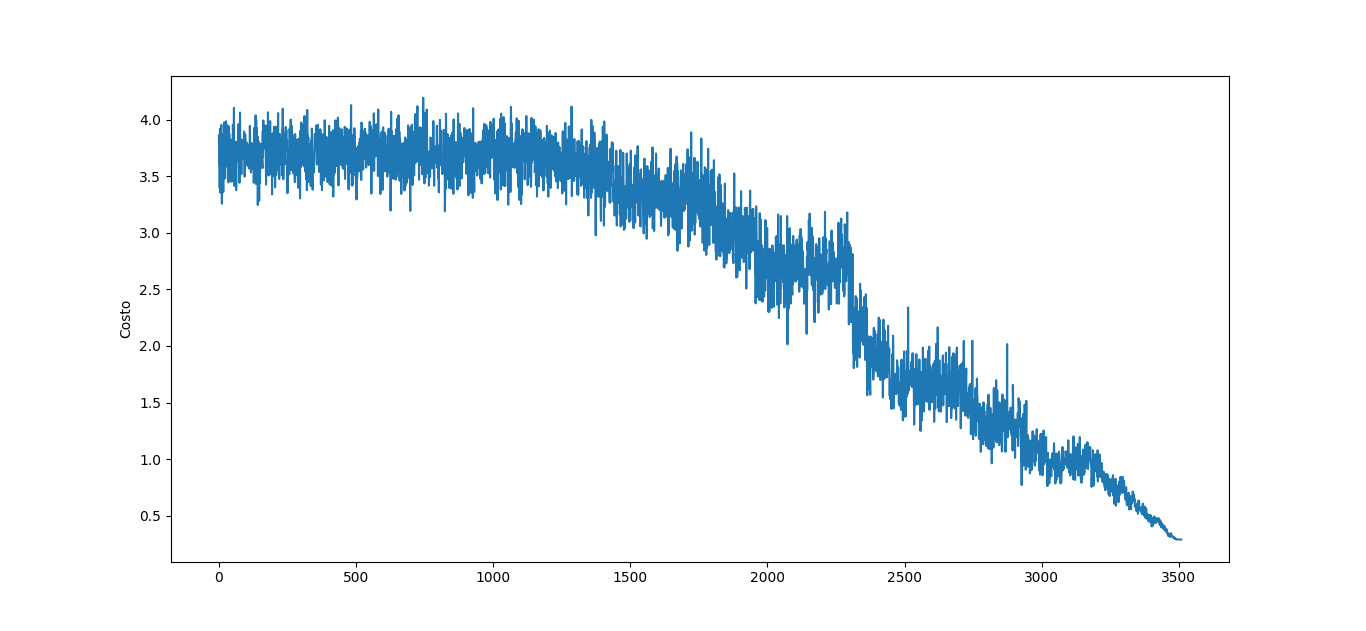
\includegraphics[width=10cm, height=8cm]{grafica}
\end{center}
Esta fue la mejor soluci�n obtenida con dicho conjunto. El costo final es de 0.28963322352405946 y la soluci�n es factible. Se obtuvo con la semilla 72.
El programa para generar estas gr�ficas se encuentra en la carpeta \textit{graficas}. Est� escrito en python y toma como entrada un archivo con el costo de una soluci�n por l�nea con el formato
\begin{verbatim}
E: <costo>
\end{verbatim}

\section{Conclusiones}
\begin{itemize}
\item Aunque la heur�sitica no es dif�cil de programar en s�, pueden ocurrir varios errores durante el proceso, as� que hay que hacerlo con cuidado.
\item Me falta hacer m�s experimentaci�n sobre los par�metros.
\item El proyecto fue muy divertido.
\end{itemize}

\end{document}
 
 
